\begin{tikzpicture}
\visible<2>{
	\node[] () at (-0.2, 0.2) {
\includegraphics[width=5.5cm]{Diapos/Intro/Figures/photo_camera_1}};
	}
	\node[] () at (4.3,0.2) {\begin{tikzpicture}[scale=0.79]
		\tikzstyle{every pin edge}=[<-,shorten <=1pt]
		\tikzstyle{neuron}=[circle,fill=black!25,minimum size=17pt,inner sep=0pt]
		\tikzstyle{input neuron}=[neuron,draw=black,fill=red!80!black];
		\tikzstyle{output neuron}=[neuron,draw=black,fill=blue!80!black];
		\tikzstyle{hidden neuron}=[neuron,draw=black,fill=yellow!50!orange];
		\tikzstyle{annot} = [text width=4em, text centered]
			
			% Draw the input layer nodes
		\foreach \name / \y in {1,...,4}
		% This is the same as writing \foreach \name / \y in {1/1,2/2,3/3,4/4}
		\node[input neuron] (I-\name) at (0,-\y) {}; %{$\bf n$};
			
			% Draw the hidden layer nodes
		\foreach \name / \y in {1,...,5}
		\path[yshift=0.5cm]
		node[hidden neuron] (H-\name) at (\layersep,-\y cm) {}; %{$\bf n$};
			
			% Draw the hidden layer nodes
		\foreach \name / \y in {1,...,5}
		\path[yshift=0.5cm]
		node[hidden neuron] (H2-\name) at (\layersep+\layersep,-\y cm) {}; %{$\bf n$};
			
			
			% Draw the output layer node
		\foreach \name / \y in {1,...,3}
		\path[yshift=-0.5cm]
		node[output neuron] (O-\name) at (\layersep+\layersep+\layersep,-\y cm) {}; %{$\bf n$};
			
			% Connect every node in the input layer with every node in the
			% hidden layer.
		\foreach \source in {1,...,4}
		\foreach \dest in {1,...,5}
		\path (I-\source) edge (H-\dest);
			
		\foreach \source in {1,...,5}
		\foreach \dest in {1,...,5}
		\path (H-\source) edge (H2-\dest);
			
			% Connect every node in the hidden layer with the output layer
		\foreach \source in {1,...,5}
		\foreach \dest in {1,...,3}
		\path (H2-\source) edge (O-\dest);

%	    \node[] () at (0.75, -.4) {$A_1$};	
%		\node[] () at (2.25, -0.2) {$A_2$};
%		\node[] () at (3.85,-.7) {$A_3$};
			% Annotate the layers
		\end{tikzpicture}};

	\node[] () at (4.3, 2.8) {Neural Network};
\visible<2>{		
	\node[] () at (8.8, 1.2) {
\includegraphics[trim={0 10cm 0 20cm},clip,width=2.5cm]{Diapos/Intro/Figures/cat}};
	\node[] () at (8.8,-1) {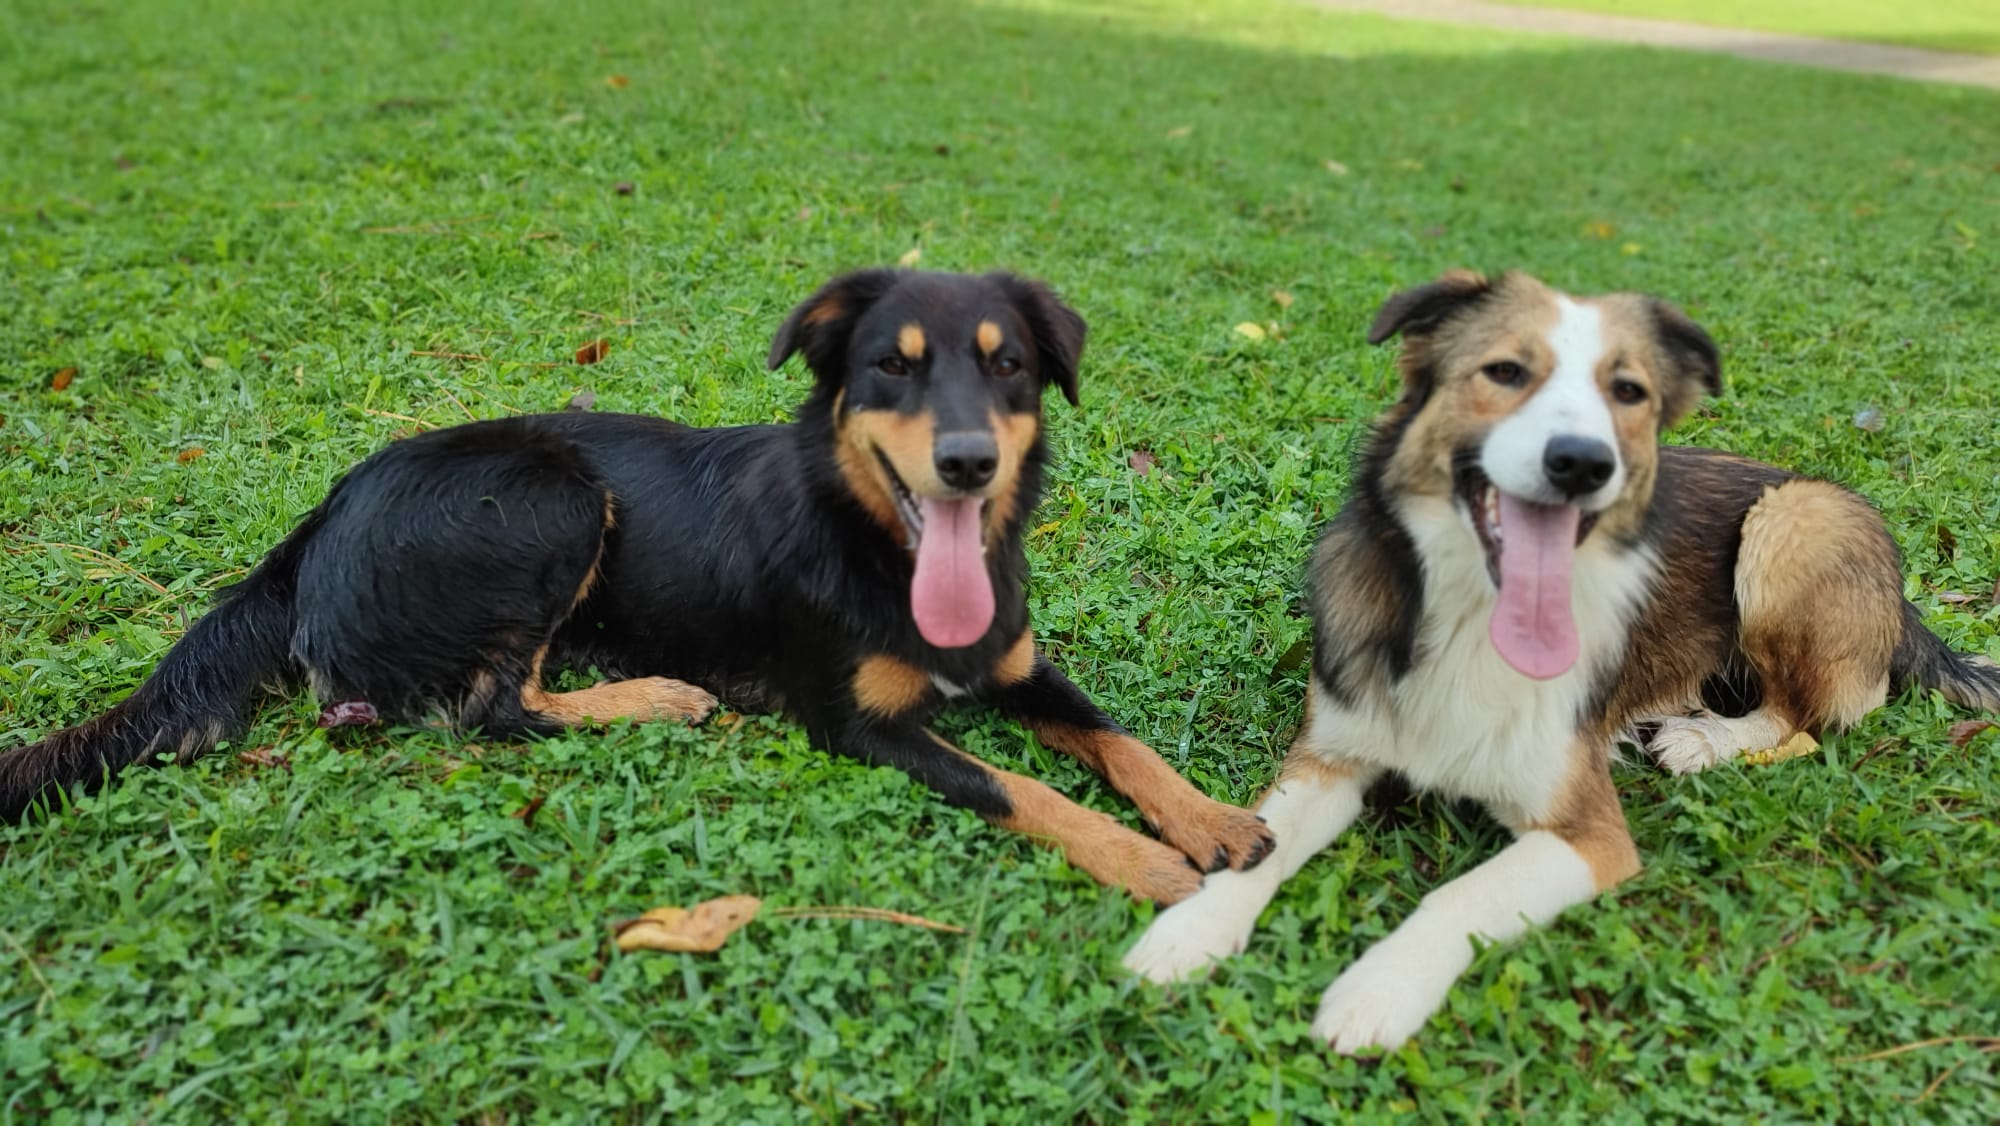
\includegraphics[width=2.5cm,height=2cm]{Diapos/Intro/Figures/dog}};
	\node[] () at (8.4, 2.8) {Output};
	\node[] () at (0, 2.8) {Input};
		
	\draw [decorate,very thick,decoration={brace,amplitude=10pt},xshift=-4pt,yshift=0pt]
		(1.3,1.5) -- (1.3,-1.5);
	\draw [decorate,very thick,decoration={brace,amplitude=10pt},xshift=-4pt,yshift=0pt]
		(7.5,-2) -- (7.5,2);
	
	}	
\end{tikzpicture}